\documentclass[tikz]{standalone}
\standaloneconfig{border=1cm} 
\usepackage[utf8]{inputenc}

\usetikzlibrary{calc}

\title{Weight Sharing in CNNs}
\author{James Allingham}
\date{April 2019}

\begin{document}

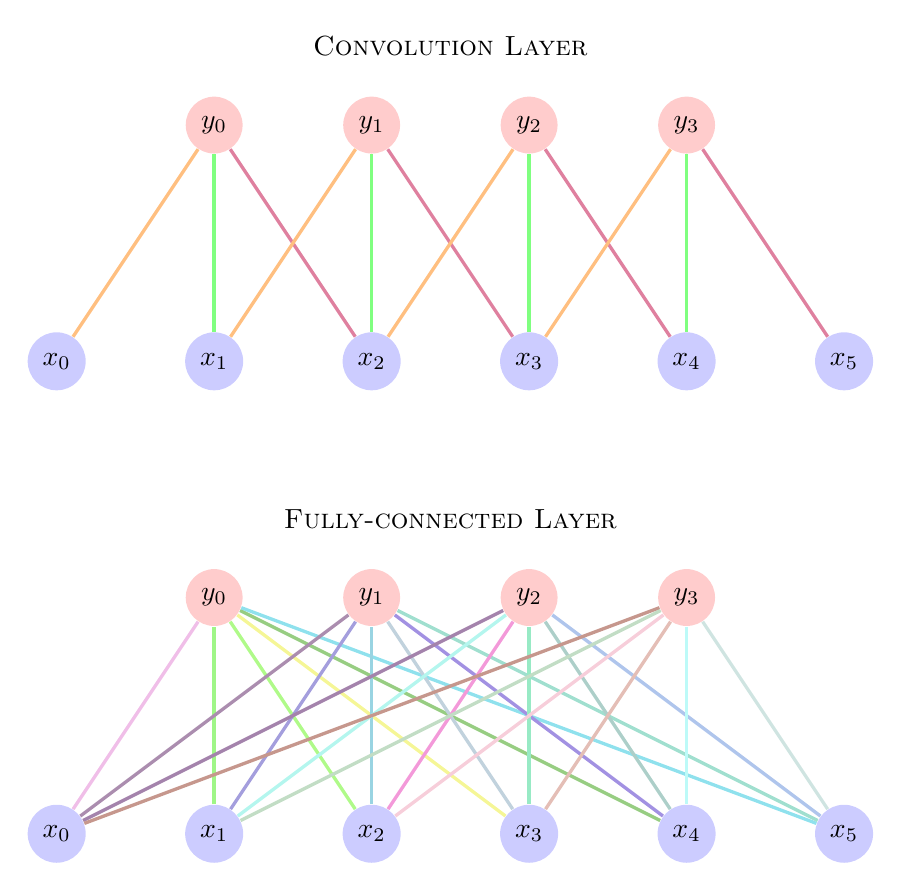
\begin{tikzpicture}
    % \draw[help lines](0,-5) grid (10,5);    
    
    % Convolution Layer:
    \node[] at (5,4) {\textsc{Convolution Layer}};
    
    % input nodes
    \foreach \z in {0,1,...,5} {
        \node[circle, fill=blue!20, label={}, minimum size=0.5cm] (z\z) at ($2*(\z,0)$) {$x_{\z}$};
    }
    
    % output nodes and edges
    \foreach \y in {0,1,...,3} {
        \node[circle, fill=red!20, label={}, minimum size=0.5cm] (y\y) at ($2*(\y,0) + (2,3)$) {$y_{\y}$};
        \pgfmathsetmacro{\prev}{\y};
        \pgfmathtruncatemacro{\cur}{\y + 1};
        \pgfmathtruncatemacro{\next}{\y + 2};
        \path[draw=orange!50, very thick] (z\prev) edge[-] (y\y);
        \path[draw=green!50, very thick] (z\cur) edge[-]  (y\y);
        \path[draw=purple!50, very thick] (z\next) edge[-] (y\y);
    }
    
    % Fully-connected Layer
    \node[] at (5,-2) {\textsc{Fully-connected Layer}};
    
    % input nodes
    \foreach \a in {0,1,...,5} {
        \node[circle, fill=blue!20, label={}, minimum size=0.5cm] (a\a) at ($2*(\a,0) + (0,-6)$) {$x_{\a}$};
    }
    
    % output nodes and edges
    \foreach \b in {0,1,...,3} {
        \node[circle, fill=red!20, label={}, minimum size=0.5cm] (b\b) at ($2*(\b,0) + (2,-3)$) {$y_{\b}$};
        \foreach \a in {0,1,...,5} {
            \edef\R{\pdfuniformdeviate 255}
            \edef\G{\pdfuniformdeviate 255}
            \edef\B{\pdfuniformdeviate 255}
            \xdefinecolor{MyColor}{RGB}{\R,\G,\B}
            \path[draw=MyColor!50, very thick] (a\a) edge[-] (b\b);
        }
    }

\end{tikzpicture}

\end{document}
